\documentclass[letterpaper, 12pt]{article}

\usepackage[top=2.5cm, bottom=2.5cm, left=2cm, right=2cm]{geometry}
\usepackage{amsmath, amsfonts, amssymb, amsthm}
\usepackage{graphicx}

\def\e{\text{e}}

\title{Solving parabolic PDEs in parallel via time discretization using Laplace transforms}
\author{Kyle Geyser and Dylan Denning}
\date{\today}

\begin{document}
 \maketitle
 
 % nice mathy stuff for our presentation
 
 $$U_{N,\tau}(t)=2\text{Re}\left(\frac{1}{N\tau}\sum_{j=0}^{N-1}{}^\prime \tilde{\mu_j}\e^{z_jt}w(z_j)\right)$$
 $$(zI+A)w(z)=u_0+\hat{f}(z)$$
 $$u_t+Au=f(t),\hspace{4mm}\text{for }t>0,\hspace{4mm}\text{with }u(0)=u_0$$
 $$u_t-u_{xx}=f(x,t),\hspace{4mm}\text{for }0<x<\pi,\;t>0,$$
 $$u(x,t)=0\hspace{4mm}\text{for }x=0\text{ and }\pi,\;t>0,\hspace{4mm}\text{with }u(x,0)=u_0(x),\hspace{4mm}\text{for }0<x<\pi$$
 $$u(x,t)=(1+t)\e^{-t}\sin(x)+\cos(t)\e^{-2t}\sin(2x)$$
 $$u_0(x)=\sin(x)+\sin(2x)$$
 $$\hat{f}(x,z)=\frac{1}{1+z}\sin(x)+\frac{2z+3}{(z+2)^2+1}\sin(2x)$$
 
 % end nice mathy stuff
	
	\section*{Summary}
	\hspace{5mm} In a normal space-time setting, partial differential equations can be impossible to solve using parallel methods. For each unit of time, the unknown function relies on the values at previous times. Given a parabolic PDE, one can transform the problem into many discrete, space-frequency problems, independent of one another. Following this transformation, parallel methods can be applied to solving the problem with high speed and accuracy. The methods used in this project can be applied to many fields involving differential equations in time, reducing the time needed to solve problems which previously could only be solved with a serial mentality.
	
	\section*{Project Description}
	\subsection*{Aims and Background}
	\hspace{5mm} The aim of this project is to produce a working program for numerically approximating solutions to space-time differntial equations. We will use a Laplace transform to transform the problem from temporal space into a frequency space. Aiding us in our research and development of this project is an article\cite{sheen03} written in the IMA Journal of Numerical Analysis on the subject matter. We will attempt to replicate the results gained by the authors in this article.
	
	\subsection*{Approach and Methodology}
	\hspace{5mm} We will begin our studies with producing a working serial version of the algorithm for ordinary differential equations with known solutions, with which we can then compare computed results. Following successful completion of said serial algorithm, we will make the necessary adjustments as to allow for partial differential equation computations, still performing all computations in serial. Once a fully working serial version of the code is completed, we will proceed to parallelize the algorithm to produce our intended final result. By approaching the problem with this methodology, we can work in steps in which we feel comfortable. Between each step, should we need outside guidance, we can approach Dr. Ganesh with any problems we are having, while still showing that we are making progress toward a final production. Throughout the time spent working through these milestones, we can further our knowledge on the subject matter by continuing to digest more of the material in the provided article\cite{
sheen03} as well as learn new material in the field of numerical solutions to PDEs through Dr. Ganesh's private lectures.
	
	\subsection*{Expected Outcome}
	\hspace{5mm} Since we are replicating the process in the article by Sheen, Sloan, and Thom\'{e}e, we expect to get the same results the authors show in section 6 (Numerical examples) in their paper.\cite{sheen03}
	
	\subsection*{Tables and Plots}
	
	\begin{tabular}{r|rrrrrrr}
		  t        &e\_10        &e\_20        &p\_20        &e\_40        &p\_40        &e\_80        &p\_80 \\ 
		\hline
		0.2    &3.715E-04    &2.018E-04         &0.88    &3.574E-04        &-0.82    &3.451E-04         &0.05 \\ 
		0.4    &4.808E-04    &1.654E-04         &1.54    &3.972E-05         &2.06    &1.710E-06         &4.54 \\ 
		0.6    &1.704E-05    &2.586E-05        &-0.60    &9.553E-06         &1.44    &1.705E-06         &2.49 \\ 
		0.8    &1.441E-05    &1.837E-07         &6.29    &1.175E-06        &-2.68    &3.131E-07         &1.91 \\ 
		1.0    &9.086E-06    &1.158E-06         &2.97    &4.299E-08         &4.75    &4.452E-08        &-0.05 \\ 
		1.2    &1.480E-06    &2.628E-07         &2.49    &2.781E-08         &3.24    &5.071E-09         &2.46 \\ 
		1.4    &5.214E-06    &2.419E-08         &7.75    &9.365E-09         &1.37    &2.872E-10         &5.03 \\ 
		1.6    &9.582E-06    &2.534E-08         &8.56    &1.248E-09         &4.34    &6.188E-11         &4.33 \\ 
		1.8    &1.545E-05    &7.777E-09        &10.96    &1.674E-10         &5.54    &2.650E-11         &2.66 \\ 
		2.0    &2.305E-05    &7.890E-09        &11.51    &1.221E-10         &6.01    &5.444E-12         &4.49 \\ 
		3.0    &9.117E-05    &2.193E-08        &12.02    &1.247E-13        &17.42    &6.523E-16         &7.58 \\ 
		4.0    &2.640E-04    &6.540E-08        &11.98    &5.787E-15        &23.43    &6.939E-18         &9.70 \\ 
	\end{tabular}
	
	\begin{tabular}{r|rrr|rrr}
							 &Tau = 0.25   &						 &						 &Tau = 1.0		 &						 &		  \\
		\hline
		  t        &e\_40        &e\_80        &p\_80        &e\_40        &e\_80        &p\_80 \\ 
		\hline
		0.2    &1.954E-05    &6.513E-07         &4.91    &4.940E-03    &2.792E-03         &0.82 \\ 
		0.4    &4.151E-07    &1.258E-07         &1.72    &1.344E-03    &1.060E-03         &0.34 \\ 
		0.6    &9.456E-09    &1.612E-09         &2.55    &7.211E-04    &3.211E-04         &1.17 \\ 
		0.8    &7.712E-10    &2.510E-11         &4.94    &6.373E-05    &2.477E-05         &1.36 \\ 
		1.0    &4.394E-10    &1.504E-12         &8.19    &6.359E-05    &3.183E-05         &1.00 \\ 
		1.2    &4.342E-10    &2.195E-14        &14.27    &2.678E-05    &3.323E-06         &3.01 \\ 
		1.4    &1.454E-09    &1.832E-15        &19.60    &8.530E-07    &2.766E-06        &-1.70 \\ 
		1.6    &2.700E-09    &4.163E-16        &22.63    &4.399E-06    &8.962E-07         &2.30 \\ 
		1.8    &4.220E-09    &4.441E-16        &23.18    &1.281E-06    &1.798E-07         &2.83 \\ 
		2.0    &6.075E-09    &5.829E-16        &23.31    &3.676E-07    &1.596E-07         &1.20 \\ 
		3.0    &2.355E-08    &2.318E-15        &23.28    &3.466E-09    &1.814E-09         &0.93 \\ 
		4.0    &7.010E-08    &6.994E-15        &23.26    &6.142E-10    &3.219E-11         &4.25 \\ 
	\end{tabular}
	
	\begin{tabular}{r|rrrrrrr}
		  t        &e\_10        &e\_20        &p\_20        &e\_40        &p\_40        &e\_80        &p\_80 \\ 
		\hline
		0.2    &1.269E-02    &2.102E-02        &-0.73    &2.381E-02        &-0.18    &2.450E-02        &-0.04 \\ 
		0.4    &2.140E-02    &8.455E-03         &1.34    &5.226E-03         &0.69    &4.416E-03         &0.24 \\ 
		0.6    &1.522E-02    &3.802E-03         &2.00    &9.256E-04         &2.04    &2.070E-04         &2.16 \\ 
		0.8    &1.212E-02    &2.912E-03         &2.06    &6.515E-04         &2.16    &8.384E-05         &2.96 \\ 
		1.0    &9.506E-03    &2.351E-03         &2.02    &6.009E-04         &1.97    &1.661E-04         &1.86 \\ 
		1.2    &7.370E-03    &1.811E-03         &2.02    &4.520E-04         &2.00    &1.141E-04         &1.99 \\ 
		1.4    &5.859E-03    &1.470E-03         &2.00    &3.650E-04         &2.01    &8.993E-05         &2.02 \\ 
		1.6    &5.148E-03    &1.276E-03         &2.01    &3.186E-04         &2.00    &7.977E-05         &2.00 \\ 
		1.8    &4.663E-03    &1.176E-03         &1.99    &2.937E-04         &2.00    &7.348E-05         &2.00 \\ 
		2.0    &4.468E-03    &1.114E-03         &2.00    &2.783E-04         &2.00    &6.958E-05         &2.00 \\ 
		3.0    &3.091E-03    &7.691E-04         &2.01    &1.927E-04         &2.00    &4.823E-05         &2.00 \\ 
		4.0    &1.825E-03    &4.533E-04         &2.01    &1.133E-04         &2.00    &2.854E-05         &1.99 \\ 
	\end{tabular}
	
	\begin{tabular}{r|rr}
		Cores              &Sayers Lab                     &Mio \\ 
	\hline
		  1.0      &3661.0877999999998      &2245.8103000000001 \\ 
		  2.0      &1918.2696000000001      &1182.6335999999999 \\ 
		  4.0               &1021.9571      &636.83158000000003 \\ 
		  8.0      &474.32260000000002               &348.26038 \\ 
		 16.0      &264.32758000000001      &164.24718999999999 \\ 
		 32.0               &153.50402      &80.234003999999999 \\ 
		 64.0      &84.893333999999996      &43.834428000000003 \\ 
		128.0                     &N/A      &21.293009999999999 \\ 
		256.0                     &N/A      &16.503080000000001 \\ 
		512.0                     &N/A      &23.166782000000001 \\ 
	\end{tabular}
	
	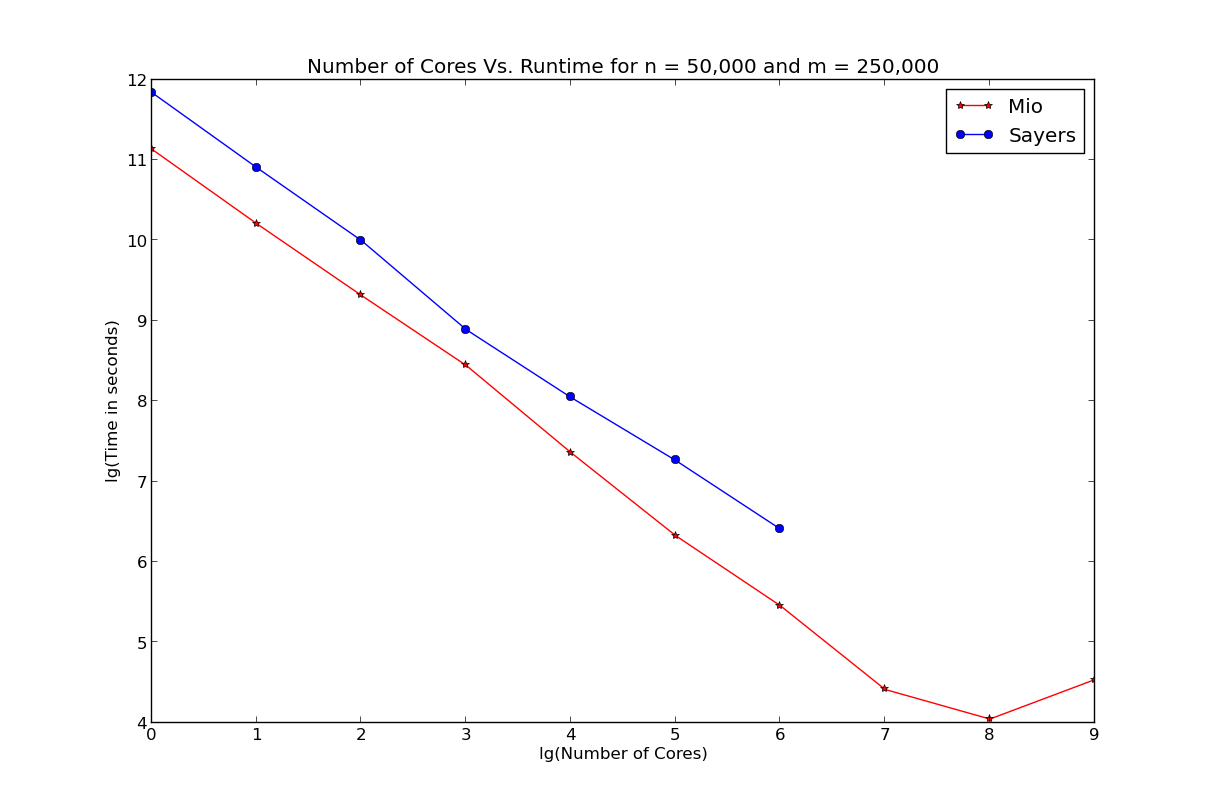
\includegraphics[width=.75\linewidth]{ProjectFiles/results/plots/coresVtime.png}
	
	\begin{tabular}{r|rr}
  Cores              &Sayers Lab                     &Mio \\ 
	\hline
		  1.0                     &1.0                     &1.0 \\ 
		  2.0      &1.9085366311388137       &1.898990777870678 \\ 
		  4.0      &3.5824280686537624      &3.5265372675142777 \\ 
		  8.0       &7.718560743257858      &6.4486528728878092 \\ 
		 16.0      &13.850570568534692      &13.673355994705298 \\ 
		 32.0      &23.850110244669814      &27.990754393860239 \\ 
		 64.0      &43.125739413179367      &51.233936484810521 \\ 
		128.0                     &N/A      &105.47171583538449 \\ 
		256.0                     &N/A      &136.08431274646915 \\ 
		512.0                     &N/A      &96.940969185966352 \\ 
	\end{tabular}
	
	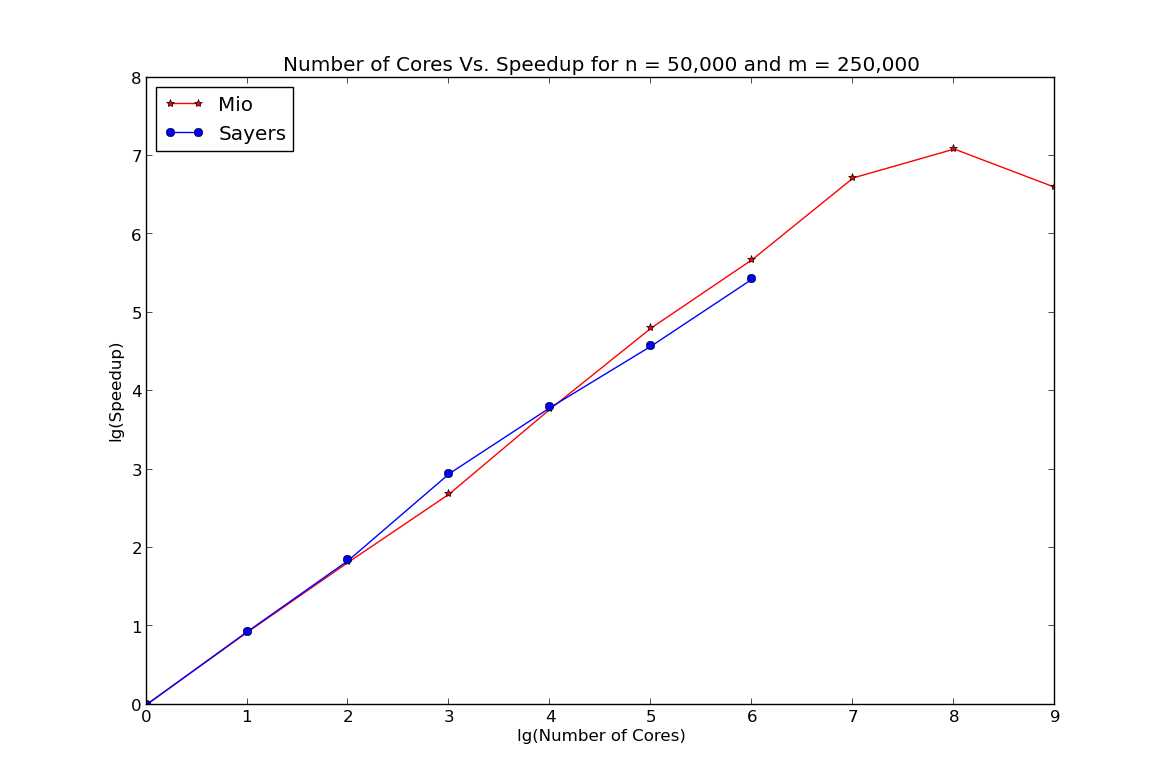
\includegraphics[width=.75\linewidth]{ProjectFiles/results/plots/coresVspeedup.png}
	
	\begin{tabular}{r|rr}
		Cores              &Sayers Lab                     &Mio \\ 
	\hline
		  1.0                     &1.0                     &1.0 \\ 
		  2.0     &0.95426831556940683     &0.94949538893533902 \\ 
		  4.0      &0.8956070171634406     &0.88163431687856941 \\ 
		  8.0     &0.96482009290723225     &0.80608160911097615 \\ 
		 16.0     &0.86566066053341828     &0.85458474966908116 \\ 
		 32.0     &0.74531594514593169     &0.87471107480813248 \\ 
		 64.0     &0.67383967833092762     &0.80053025757516438 \\ 
		128.0                     &N/A      &0.8239977799639413 \\ 
		256.0                     &N/A     &0.53157934666589512 \\ 
		512.0                     &N/A     &0.18933783044134053 \\ 
	\end{tabular}
	
	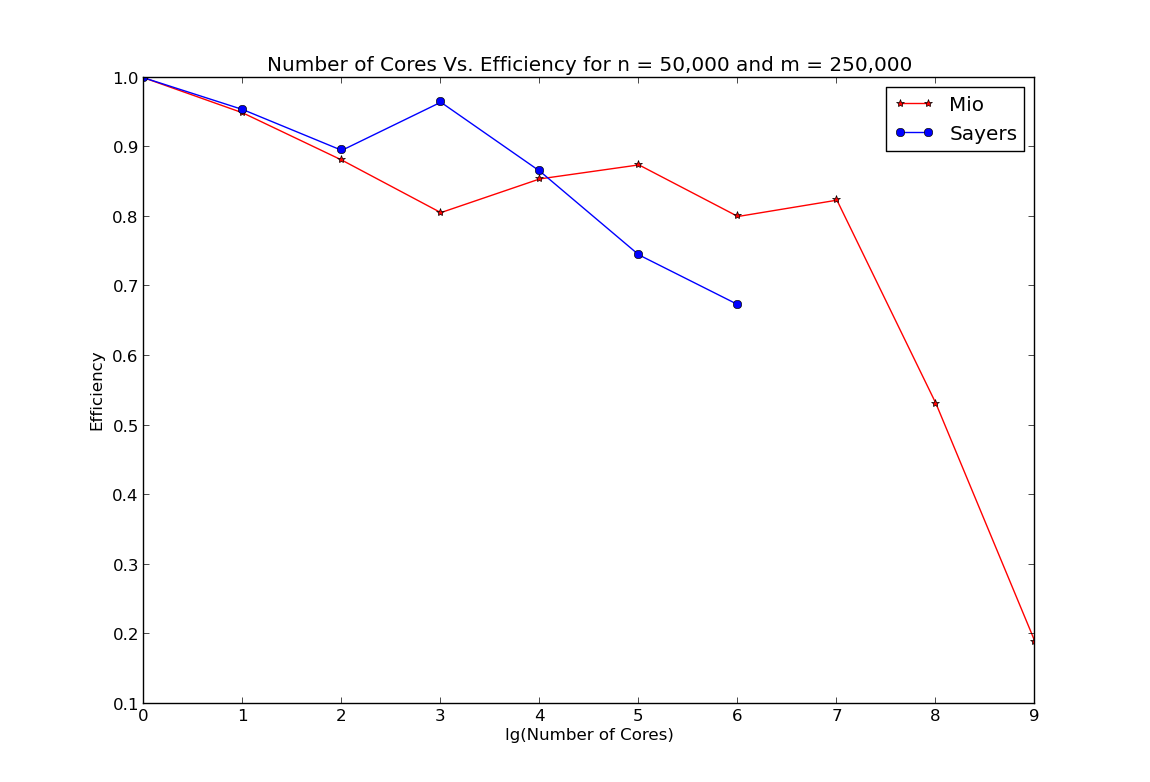
\includegraphics[width=.75\linewidth]{ProjectFiles/results/plots/coresVefficiency.png}
	
	\begin{tabular}{r|rr}
		Cores              &Sayers Lab                     &Mio \\ 
	\hline
		  2.0    &0.047923297551072164    &0.053191001929236759 \\ 
		  4.0     &0.03885371628253953    &0.044752372896321647 \\ 
		  8.0   &0.0052089514409975812    &0.034367025567564609 \\ 
		 16.0    &0.010345804508339492    &0.011343930518085162 \\ 
		 32.0     &0.01102299598743091   &0.0046204722317963586 \\ 
		 64.0   &0.0076830559693734967   &0.0039551114498611187 \\ 
		128.0                     &N/A   &0.0016818543519778373 \\ 
		256.0                     &N/A   &0.0034556341402023306 \\ 
		512.0                     &N/A   &0.0083787958735268026 \\ 
	\end{tabular}
	
	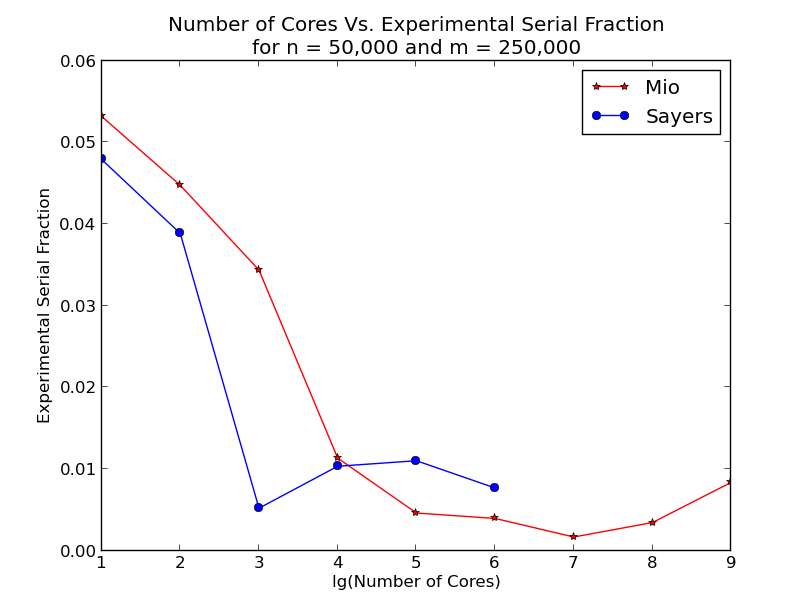
\includegraphics[width=.75\linewidth]{ProjectFiles/results/plots/coresVexpserialfrac.png}
	
	\begin{thebibliography}{1}
		\bibitem{sheen03}
			Dongwoo Sheen, Ian H. Sloan, and Vidar Thom\'{e}e,
			\emph{A parallel method for time discretization of parabolic equations based on Laplace transformation and quadrature}.
			IMA Journal of Numerical Analysis (2003) 23,
			269-299
			
	\end{thebibliography}

\end{document}
